\documentclass[tikz,border=10pt]{standalone}
\usetikzlibrary{shapes, backgrounds, arrows.meta}

\begin{document}
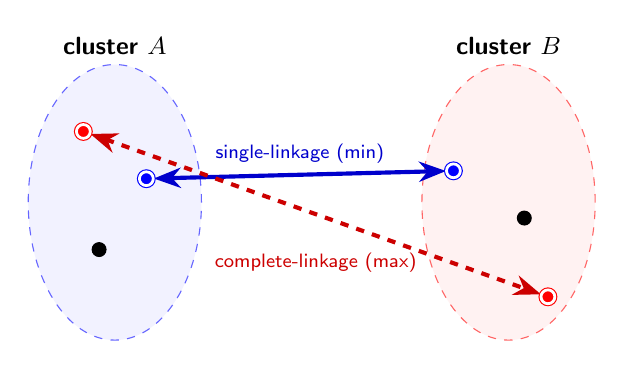
\begin{tikzpicture}[
    point/.style={circle, draw, fill=black, inner sep=0pt, minimum size=5pt},
    cluster/.style={ellipse, draw, dashed, minimum width=2.2cm, minimum height=3.5cm, inner sep=5pt},
    label style/.style={font=\sffamily\small\bfseries}
]

    % --- KLASTER A (Lewy) ---
    \node[cluster, fill=blue!5, draw=blue!60, label={[label style]above:cluster $A$}] (cA) at (0,0) {};
    \node[point] (a1) at (-0.4, 0.9) {};
    \node[point] (a2) at (0.4, 0.3) {};
    \node[point] (a3) at (-0.2, -0.6) {};

    % --- KLASTER B (Prawy) ---
    \node[cluster, fill=red!5, draw=red!60, label={[label style]above:cluster $B$}] (cB) at (5,0) {};
    \node[point] (b1) at (4.3, 0.4) {};
    \node[point] (b2) at (5.2, -0.2) {};
    \node[point] (b3) at (5.5, -1.2) {};

    % --- SINGLE-LINKAGE (Najbliższe sąsiedztwo) ---
    % Połączenie między najbliższymi punktami: a2 oraz b1
    \draw[line width=1.5pt, blue!80!black, <->, >=Stealth] (a2) -- (b1) 
        node[midway, above, font=\sffamily\scriptsize, text=blue!80!black] {single-linkage (min)};

    % --- COMPLETE-LINKAGE (Najdalsze sąsiedztwo) ---
    % Połączenie między najdalszymi punktami: a1 oraz b3
    \draw[line width=1.5pt, red!80!black, dashed, <->, >=Stealth] (a1) -- (b3) 
        node[midway, below=10pt, font=\sffamily\scriptsize, text=red!80!black] {complete-linkage (max)};

    % Podświetlenie kluczowych punktów dla czytelności (Poprawione)
    \draw[white, fill=blue, draw=blue, double, double distance=1pt] (a2) circle (2.5pt);
    \draw[white, fill=blue, draw=blue, double, double distance=1pt] (b1) circle (2.5pt);
    
    \draw[white, fill=red, draw=red, double, double distance=1pt] (a1) circle (2.5pt);
    \draw[white, fill=red, draw=red, double, double distance=1pt] (b3) circle (2.5pt);

\end{tikzpicture}
\end{document}

